% !TEX encoding = UTF-8 Unicode
%%
%%		XX_名前_日付.{tex,pdf}
%%		XX, 名前, 日付は naming rule に従う
%%
\documentclass[11pt,a4paper]{jsarticle}

%% ページ設定のパラメータは変更しない
\usepackage[top=72pt,bottom=60pt,left=40pt,right=40pt]{geometry}
\setlength{\topmargin}{-38pt}
\setlength{\headheight}{18pt}
\setlength{\headsep}{20pt}
\setlength{\footskip}{38pt}
\setlength{\topskip}{0pt}
%%

%% 共通フォーマット
\usepackage{fancyhdr}
\rhead{\stdid, \sirname}
\cfoot{}
\rfoot{\thepage}
\renewcommand{\footrulewidth}{\headrulewidth}
\pagestyle{fancy}

\usepackage{subfig}
\usepackage{layout}

%% \title{maketitleは使わない}
%% \author{}
%% \date{}

%% 自分の使うパッケージ
\usepackage{amsmath,amssymb}
\usepackage{bm}
\usepackage[dvipdfmx]{graphicx}
\usepackage{ascmac}
\usepackage{indentfirst}
\graphicspath{{./images/}}

%% 個人設定、日付設定
\lfoot{2019年 8月20日}		%% 日付
\def\stdid{18T0006}		%% 学生証番号
\def\sirname{小室}		%% 姓
\def\firstname{光広}		%% 名


\begin{document}
%% \maketitle			%% maketitle は使わない

\noindent
\textbf{\large 進捗レポート (\stdid, \sirname\ \firstname)}		%%  固定

%%
\section*{今週の進捗サマリ}			%% 固定

\begin{itemize}
\item 最終面接に向けた準備
\item CartPole-v0のPyTorch実装
\end{itemize}

%%
\section{進捗詳細}					%% 固定
\subsection{最終面接に向けた準備}
8月21日に行われる最終面接の準備を行っていた.具体的には,想定質問の作成,キャリアセンターでの相談・模擬面接
などである.学校推薦を使用しているが,通常の選考と変わることなく全力で臨みたい.

\subsection{CartPole-v0のPyTorch実装}
強化学習のHello world的タスクである\texttt{Open AI Gym}の\texttt{Atari CartPole-v0}を
\texttt{PyTorch}により実装した.本タスクは左右に動かせる台を使い上に立つ棒をいかに倒さずに動かす
事ができるかを学ぶタスクである.今週は本タスクをPyTorchにより実装し,ローカルの\texttt{Jupyter Lab}
上と\texttt{Colaboratory}上で動作させた.コードはマイナビより出版されている本\cite{book1}を使用した.
\texttt{Colaboratory}上で動作させた結果を図1に示す.
\begin{figure}[htbp]
  \begin{center}
    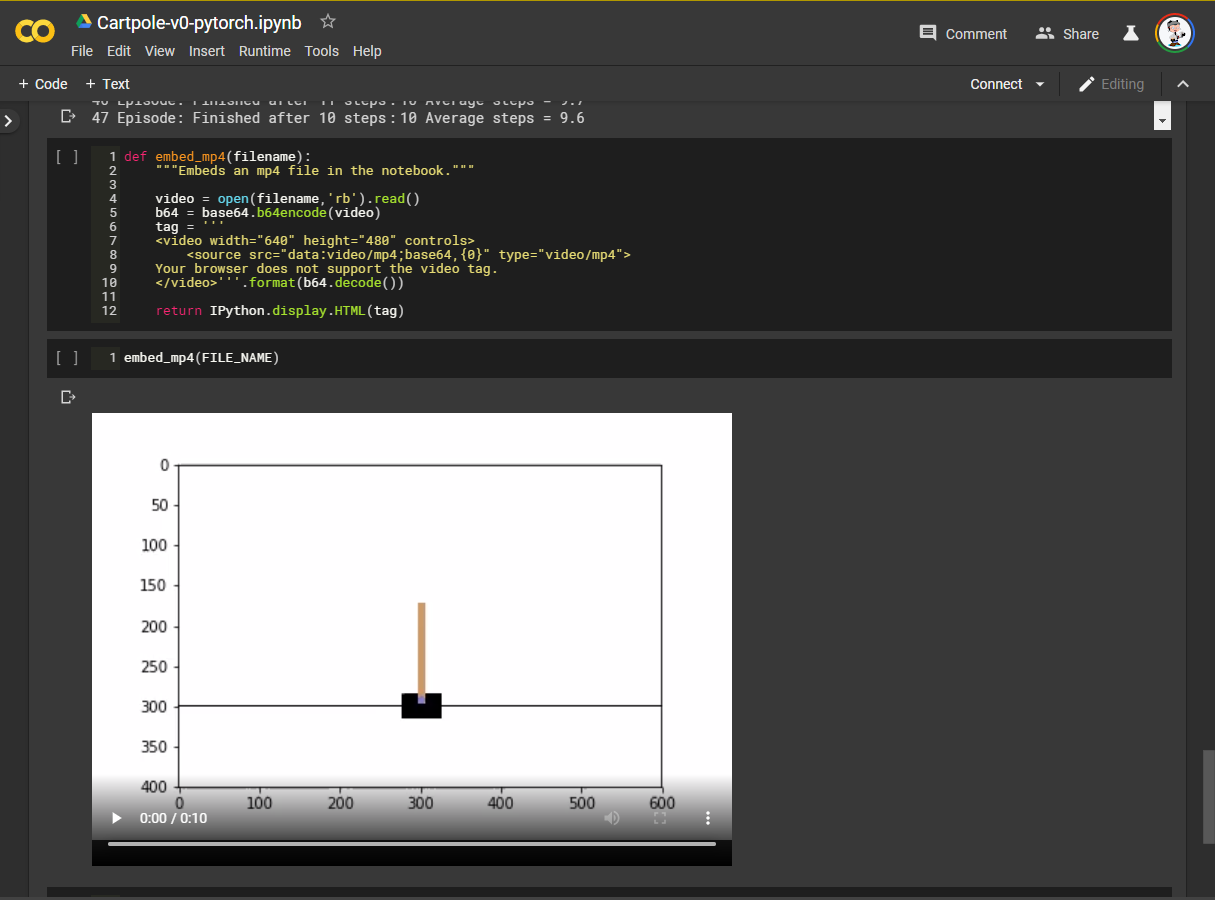
\includegraphics[width=14cm]{fig1.png}
    \caption{\texttt{CartPole-v0}の実行結果}
  \end{center}
  \label{fig1}
\end{figure}
図1では\texttt{Colaboratory}の\texttt{ipnb}ノートブック上に学習結果の動画を出力した画像である.
\texttt{Colaboratory}は特殊環境(Google Compute Engine上のコンテナであるためGUI処理に追加処理が必要)
であるため,動画埋め込み出力の実装に時間がかかってしまっていた.


\section{今後の予定}
今回は単純にローカル環境と\texttt{Colaboratory}上で動作確認を行っただけであるため,コードの理解を含め,
\texttt{Breakout}の実装へ入りたい.なお,\texttt{PyTorch}による実装では,学習ループを自前で用意するため,
Sync型(仮称)案を比較的簡単に実装できると考えている.現時点では,\texttt{Agent} Classを複数持つリストで順に
1サイクル実行,各\texttt{Agent}で評価値(Reward)が最も高い\texttt{Agent}を選択することなどを考えている.
メインの庵であるDurabilityについては,特定エピソード数Reward値が上昇しないあるいは下降した場合,そのAgentの
Durable valueを減少させることなどを想定している.

\begin{thebibliography}{1}
  \bibitem{book1} 小川雄太郎,つくりながら学ぶ!深層強化学習 PyTorchによる実践プログラミング,マイナビ出版,2018
\end{thebibliography}

\end{document}

